\achapter{17}{The Determinant} \label{chap:determinants}

\vspace*{-17 pt}
\framebox{
\parbox{\dimexpr\linewidth-3\fboxsep-3\fboxrule}
{\begin{fqs}
\item How do we calculate the determinant of an $n \times n$ matrix?
\item What is one important fact the determinant tells us about a matrix?

\end{fqs}}}% \hspace*{3 pt}}

\vspace*{13 pt}

\csection{Application: Area and Volume}       % Enter section title between curly braces
\label{sec:appl_area_vol}
Consider the problem of finding the area of a parallelogram determined by two  vectors $\vu$ and $\vv$, as illustrated at left in Figure \ref{F:det_area}.
\begin{figure}[ht]
  \begin{center}
\resizebox{!}{1.15in}{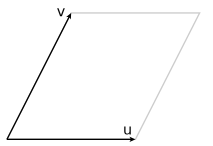
\includegraphics{det_area_2.eps}} \hspace{0.1in} \resizebox{!}{1.15in}{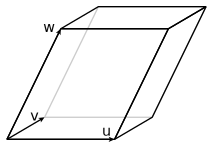
\includegraphics{det_volume_2.eps}}
    \caption{A parallelogram and a parallelepiped.}
    \label{F:det_area}
  \end{center}
\end{figure}
We could calculate this area, for example, by breaking up the parallelogram into two triangles and a rectangle and finding the area of each. Now consider the problem of calculating the volume of the three-dimensional analog (called a \emph{parallelepiped}) determined by three vectors $\vu$, $\vv$, and $\vw$ as illustrated at right in Figure \ref{F:det_area}. 

It is quite a bit more difficult to break this parallelepiped into subregions whose volumes are easy to compute. However, all of these computations can be made quickly by using determinants. The details are later in this section. 

\csection{Introduction}
\label{sec:det_intro}
We know that a non-zero vector $\vx$ is an eigenvector of an $n \times n$ matrix $A$ if $A \vx = \lambda \vx$ for some scalar $\lambda$. Note that this equation can be written as $(A-\lambda I_n)\vx=\vzero$. Until now, we were given eigenvalues of matrices and have used the eigenvalues to find the eigenvectors. In this section we will learn an algebraic technique to find the eigenvalues ourselves. We will also be able to justify why an $n\times n$ matrix has at most $n$ eigenvalues. 

A scalar $\lambda$ is an eigenvalue of $A$ if $(A - \lambda I_n)\vx=\vzero$ has a non-trivial solution $\vx$, which happens if and only if $A-\lambda I_n$ is not invertible. In this section we will find a scalar whose value will tell us when a matrix is invertible and when it is not, and use this scalar to find the eigenvalues of a matrix. 


\begin{pa} \label{pa:4_a} In this activity, we will focus on $2\times 2$ matrices. Let $A = \left[ \begin{array}{cc} a&b \\ c&d \end{array} \right]$ be a $2\times 2$ matrix. To see if $A$ is invertible, we row reduce $A$ by replacing row 2 with $a\cdot $(row 2) $- c \cdot $(row 1):
\[\left[ \begin{array}{cc} a&b \\ 0&ad-bc \end{array} \right].\]
So the only way $A$ can be reduced $I_2$ is if $ad - bc \neq 0$. We call this quantity $ad-bc$ the \emph{determinant} of $A$, and denote the determinant of $A$ as $\det(A)$ or $|A|$. When $\det(A)\neq 0$, we know that 
\[A^{-1} = \frac{1}{ad-bc} \left[ \begin{array}{rr} d&-b \\ -c&a \end{array} \right].\]
We now consider how we can use the determinant to find eigenvalues and other information about the invertibility of a matrix. 
\be
\item Let $A = \left[ \begin{array}{cc} 1&2 \\ 2&4 \end{array} \right]$. Find $\det(A)$ by hand. What does this mean about the matrix $A$? Can you confirm this with other methods? 



\item One of the eigenvalues of $A=\left[ \begin{array}{cc} 1&3 \\ 2&2 \end{array} \right]$ is $\lambda=4$. Recall that we can rewrite the matrix equation $A\vx=4\vx$ in the form $(A-4I_2) \vx = \vzero$. What must be true about $A-4I_2$ in order for 4 to be an eigenvalue of $A$? How does this relate to $\det(A-4I_2)$? 


\item Another eigenvalue of $A=\left[ \begin{array}{cc} 1&3 \\ 2&2 \end{array} \right]$ is $\lambda=-1$. What must be true about $A+I_2$ in order for $-1$ to be an eigenvalue of $A$? How does this relate to $\det(A+I_2)$? 



\item To find the eigenvalues of the matrix $A=\left[ \begin{array}{cc} 3&2\\2&6 \end{array} \right]$, we rewrite the equation $A \vx = \lambda \vx$ as $(A - \lambda I_2) \vx = \vzero$. The coefficient matrix of this last system has the form $A-\lambda I_2 = \left[ \begin{array}{cc} 3-\lambda &2 \\ 2& 6-\lambda \end{array} \right]$. The determinant of this matrix is a quadratic expression in $\lambda$. Since the eigenvalues will occur when the determinant is 0, we need to solve a quadratic equation. Find the resulting eigenvalues. (Note: One of the eigenvalues is 2.)



\item Can you explain why a $2\times 2$ matrix can have at most two eigenvalues?
	

\ee

\end{pa}



\csection{The Determinant of a Square Matrix}
\label{sec:det_square}

Around 1900 or so determinants were deemed much more important than they are today. In fact, determinants were used even before matrices. According to Tucker\footnote{Tucker, Alan. (1993). The Growing Importance of Linear Algebra in Undergraduate Mathematics. \emph{The College Mathematics Journal}, 1, 3-9.} determinants (not matrices) developed out of the study of coefficients of systems of linear equations and were used by Leibniz 150 years before the term matrix was coined by J. J. Sylvester in 1848. Even though determinants are not as important as they once were, the determinant of a matrix is still a useful quantity. We saw in Preview Activity \ref{pa:4_a} that the determinant of a matrix tells us if the matrix is invertible and how it can help us find eigenvalues. In this section, we will see how to find the determinant of any size matrix and how to use this determinant to find the eigenvalues.

The determinant of a $2 \times 2$ matrix $A = \left[ \begin{array}{cc} a&b \\ c&d \end{array} \right]$ is $\det(A)=ad-bc$. The matrix $A$ is invertible if and only if $\det(A) \neq 0$. We will use a recursive approach to find the determinants of larger size matrices building from the $2\times 2$ determinants. We present the result in the $3 \times 3$ case here -- a more detailed analysis can be found at the end of this section. 

To find the determinant of a $3 \times 3$ matrix $A = \left[ \begin {array}{ccc} a_{11}&a_{12}&a_{13} \\ a_{21}&a_{22}&a_{23}\\ a_{31}&a_{32}&a_{33}\end {array} \right]$, we will use the determinants of three $2\times 2$ matrices. More specifically, the determinant of $A$, denoted $\det(A)$ is the quantity
\begin{equation} \label{eq:det_3by3}
a_{11} \det\left(\left[ \begin{array}{cc} a_{22}&a_{23} \\ a_{32}&a_{33} \end{array} \right] \right)- a_{12} \det \left(\left[ \begin{array}{cc} a_{21}&a_{23} \\ a_{31}&a_{33} \end{array} \right] \right) + a_{13} \det \left(\left[ \begin{array}{cc} a_{21}&a_{22} \\ a_{31}&a_{32} \end{array} \right] \right).
\end{equation}
This sum is called a \emph{cofactor expansion} of the determinant of $A$. The smaller matrices in this expansion are obtained by deleting certain rows and columns of the matrix $A$. In general, when finding the determinant of an $n\times n$ matrix, we find determinants of $(n-1)\times (n-1)$ matrices, which we can again reduce to smaller matrices to calculate.

We will use the specific matrix 
\[ A = \left[ \begin{array}{ccc} 1 & 2 & 0 \\ 1 & 4 & 3 \\ 2 & 2 & 1\end{array} \right] \]
as an example in illustrating the cofactor expansion method in general.

\begin{itemize}
\item We first pick a row or column of $A$. We will pick the first row of $A$ for this example.

\item For each entry in the row (or column) we choose, in this case the first row, we will calculate the determinant of a smaller matrix obtained by removing the row and the column the entry is in. Let $A_{ij}$ be the smaller matrix found by deleting the $i$th row and $j$th column of $A$. For entry $a_{11}$, we find the matrix $A_{11}$ obtained by removing first row and first column:
\[A_{11} = \left[ \begin{array}{cc} 4 & 3 \\ 2 & 1 \end{array} \right]\, .\]
For entry $a_{12}$, we find
\[ A_{12} = \left[ \begin{array}{cc} 1 & 3 \\ 2 & 1 \end{array} \right]\, .\] 
Finally, for entry $a_{13}$, we find
\[ A_{13} = \left[ \begin{array}{cc} 1 & 4 \\ 2 & 2 \end{array} \right] \, .\]

\item Notice that in the $3 \times 3$ determinant formula in \eqref{eq:det_3by3} above, the middle term had a (-) sign. The signs of the terms in the cofactor expansion alternate within each row and each column. More specifically, the sign of a term in the $i$th row and $j$th column is $(-1)^{i+j}$. We then obtain the following pattern of the signs within each row and column:
\[ \left[ \begin{array}{cccc} + & - & + & \cdots \\ - & + & - & \cdots \\ + & - & + & \cdots \\ \vdots & & & \end{array} \right] \]
In particular, the sign factor for $a_{11}$ is $(-1)^{1+1}=1$, for $a_{12}$ is $(-1)^{1+2}=-1$, and for $a_{13}$ is $(-1)^{1+3}=1$. 

\item For each entry $a_{ij}$ in the row (or column) of $A$ we chose, we multiply the entry $a_{ij}$ by the determinant of $A_{ij}$ and the sign $(-1)^{i+j}$. In this case, we obtain the following numbers
\[ a_{11} (-1)^{1+1} \det(A_{11})  = 1 \det \left[ \begin{array}{cc} 4 & 3 \\ 2 & 1 \end{array} \right] = 1(4-6)=-2 \]
\[ a_{12} (-1)^{1+2} \det(A_{12}) = -2 \det \left[ \begin{array}{cc} 1 & 3 \\ 2 & 1 \end{array} \right] = -2(1-6)=10 \]
\[ a_{13} (-1)^{1+3} \det(A_{13}) = 0 \]
Note that in the last calculation, since $a_{13}=0$, we did not have to evaluate the rest of the terms.

\item Finally, we find the determinant by adding all these values:
\begin{align*}
 \det(A) &= a_{11} (-1)^{1+1} \det(A_{11}) + a_{12} (-1)^{1+2} \det(A_{12}) \\
	&\qquad + a_{13} (-1)^{1+3} \det(A_{13}) \\
	&= 8.
\end{align*}

\end{itemize}

\csection{Cofactors}
\label{sec:cofactors}

We will now define the determinant of a general $n \times n$ matrix $A$ in terms of a cofactor expansion as we did in the $3 \times 3$ case. To do so, we need some notation and terminology.

\begin{itemize}
\item We let $A_{ij}$ be the submatrix of $A = [a_{ij}]$ found by deleting the $i$th row and $j$th column of $A$. The determinant of $A_{ij}$ is called the $ij$th \emph{minor}\index{matrix!minor} of $A$ or the minor corresponding to the entry $a_{ij}$.
\item Notice that in the $3 \times 3$ case, we used the opposite of the 1,2 minor in the sum. It will be the case that the terms in the cofactor expansion will alternate in sign. We can make the signs in the sum alternate by taking $-1$ to an appropriate power. As a result, we define the $ij$th \emph{cofactor}\index{cofactor} $C_{ij}$ of $A$ as
\[C_{ij} = (-1)^{i+j} \det\left(A_{ij}\right).\]
\item Finally, we define the determinant of $A$. 
\end{itemize}

\begin{definition} If $A=[a_{ij}]$ is an $n \times n$ matrix, the \textbf{determinant}\index{determinant} of $A$ is the scalar 
\[\det(A) = a_{11}C_{11} + a_{12}C_{12} + a_{13}C_{13} + \cdots + a_{1n}C_{1n}\]
where $C_{ij}= (-1)^{i+j} \det(A_{ij})$ is the $ij$-cofactor of $A$ and $A_{ij}$ is the matrix obtained by removing row $i$ and column $j$ of matrix $A$.
\end{definition}


This method for computing determinants is called the \emph{cofactor expansion} or \emph{Laplace expansion} of $A$ along the 1st row. The cofactor expansion reduces the computation of the determinant of an $n \times n$ matrix to $n$ computations of determinants of $(n-1) \times (n-1)$ matrices. These smaller matrices can be reduced again using cofactor expansions, so it can be a long and grueling process for large matrices. It turns out that we can actually take this expansion along any row or column of the matrix (a proof of this fact is given in Section \ref{sec:det_properties}). For example, the cofactor expansion along the 2nd row is  
\[\det(A) = a_{21}C_{21} + a_{22}C_{22} + \cdots + a_{2n}C_{2n}\]
and along the 3rd column the formula is
\[\det(A) = a_{13}C_{13} + a_{23}C_{23} + \cdots + a_{n3}C_{n3}.\]

Note that when finding a cofactor expansion, choosing a row or column with many zeros makes calculations easier.



\begin{activity} \label{act:4_a_1} ~
	\ba
	\item Let $A = \left[ \begin{array}{rcr} 1&2&-1 \\ -2&0&4 \\ 6&3&0  \end{array} \right]$. Use the cofactor expansion along the first row to calculate the determinant of $A$ by hand.


	\item Calculate $\det(A)$ by using a cofactor expansion along the second row where $A = \left[ \begin{array}{ccc} 1 & 4 & 2 \\ 0 & 2 & 0 \\ 2 & 5 & 3 \end{array} \right]$. 
	
	

	\item Calculate the determinant of $\left[ \begin{array}{crr} 1&-2&3 \\ 0&4&-3 \\ 0&0&8\end{array} \right]$. 
	
	
	
	\item Which determinant property can be used to calculate the determinant in part (c)? Explain how. (Determinant properties are included below for easy reference.)
	
	
	
	\item Consider the matrix $A=\left[ \begin{array}{ccc} 1 & 1 & 2 \\ 0 & 2 & 1 \\ 1 & 2 & 2 \end{array} \right]$. Let $B$ be the matrix which results when $c$ times row 1 is added to row 2 of $A$. Evaluate the determinant of $B$ by hand to check that it is equal to the determinant of $A$, which verifies one other determinant property (in a specific case).
	
	
	
	\ea

\end{activity}

As with any new idea, like the determinant, we must ask what properties are satisfied. We state the following theorem without proof for the time being. For the interested reader, the proof of many of these properties is given in Section \ref{sec:det_properties} and others in the exercises. 


\begin{theorem} \label{thm:determinant_properties} Given $n\times n$ matrices $A, B$, the following hold:

\begin{enumerate}

\item $\det (AB) = \det (A) \cdot \det (B)$, and in particular $\det
(A^k) = (\det A)^k$ for any positive integer $k$.
\item $\det (A^{\tr}) = \det (A)$.
\item $A$ is invertible if and only if $\det (A) \neq 0$.
\item If $A$ is invertible, then $\det (A^{-1}) = (\det A)^{-1}$.
\item For a $2\times 2$ matrix $A=\begin{bmatrix} a & b \\ c & d
\end{bmatrix}$, $\det (A) = ad-bc$.
\item If $A$ is upper/lower triangular, then $\det (A)$ is the product
of the entries on the diagonal.
\item The determinant of a matrix is the product of the eigenvalues,
with each eigenvalue repeated as many times as its multiplicity.
\item Effect of row operations:
\begin{itemize}
\item Adding a multiple of a row to another does NOT change the
determinant of the matrix.
\item Multiplying a row by a constant multiplies the determinant by
the same constant.
\item Row swapping multiplies the determinant by $(-1)$.
\end{itemize}
\item If the row echelon form $U$ of $A$ is obtained by adding
multiples of one row to another, and row swapping, then $\det (A)$ is
equal to $\det (U)$ multiplied by $(-1)^r$ where $r$ is the number of row
swappings done during the row reduction.
\end{enumerate}
\end{theorem}

Note that if we were to find the determinant of a $4\times 4$ matrix using the cofactor method, we will calculate determinants of 4 matrices of size $3\times 3$, each of which will require 3 determinant calculations again. So, we will need a total of 12 calculations of determinants of $2\times 2$ matrices. That is a lot of calculations. There are other, more efficient, methods for calculating determinants. For example, we can row reduce the matrix, keeping track of the effect that each row operation has on the determinant. 



\csection{The Determinant of a $3 \times 3$ Matrix}
\label{sec:det_3by3}

Earlier we defined the determinant of a $3 \times 3$ matrix. In this section we endeavor to understand the motivation behind that definition.

We will repeat the process we went through in the $2 \times 2$ case to see how to define the determinant of a $3 \times 3$  matrix. Let
\[A =  \left[ \begin {array}{ccc} a_{11}&a_{12}&a_{13} \\ a_{21}&a_{22}&a_{23}\\ a_{31}&a_{32}&a_{33}\end {array} \right].\]
To find the inverse of $A$ we augment $A$ by the $3 \times 3$ identity matrix 
\[[A \ | \ I_3] = \left[ \begin {array}{cccccc} a_{11}&a_{12}&a_{13}&1&0&0 \\ a_{21}&a_{22}&a_{23}&0&1&0 \\ a_{31}&a_{32}&a_{33}&0&0&1 \end {array} \right]\]
and row reduce the matrix (using appropriate technology) to obtain
\[\renewcommand{\arraystretch}{2.0}  \left[ \begin{array}{rrrrrr} 1&0&0&\ds \frac{a_{33}a_{22}-a_{32}a_{23}}{d}& \ds -\frac{a_{33}a_{12}-a_{32}a_{13}}{d}& \ds \frac{-a_{13}a_{22}+a_{12}a_{23}}{d} \\ 0&1&0& \ds -\frac{a_{33}a_{21}-a_{31}a_{23}}{d}& \ds \frac{a_{33}a_{11}-a_{31}a_{13}}{d}& \ds -\frac{a_{23}a_{11}-a_{21}a_{13}}{d} \\
0&0&1& \ds \frac{-a_{31}a_{22}+a_{32}a_{21}}{d}& \ds -\frac{a_{32}a_{11}-a_{31}a_{12}}{d}& \ds \frac{a_{22}a_{11}-a_{21}a_{12}}{d} \end{array} \right],\]
where 
\begin{equation} \label{eq:4_a_3by3_det}
\begin{aligned}
d = a_{33}a_{11}a_{22}&-a_{33}a_{21}a_{12}-a_{31}a_{13}a_{22} \\
	&-a_{32}a_{11}a_{23}+a_{32}a_{21}a_{13}+a_{31}a_{12}a_{23}.
\end{aligned}
\end{equation}

In this case, we can see that the inverse of the $3 \times 3$ matrix $A$ will be defined if and only if $d \neq 0$. So, in the $3 \times 3$ case the determinant of $A$ will be given by the value of $d$ in Equation (\ref{eq:4_a_3by3_det}). What remains is for us to see how this is related to determinants of $2 \times 2$ sub-matrices of $A$. 

To start, we collect all terms involving $a_{11}$ in $d$. A little algebra shows that
\[\det(A) = a_{11} \left( a_{33} a_{22} - a_{32} a_{23} \right) - a_{33} a_{21} a_{12} - a_{31} a_{13} a_{22} + a_{32}a_{21}a_{13} + a_{31} a_{12} a_{23}.\]

Now let's collect the remaining terms involving $a_{12}$:
\[\det(A) = a_{11} \left( a_{33} a_{22} - a_{32} a_{23} \right) - a_{12} \left(a_{33} a_{21} - a_{31} a_{23} \right)  - a_{31} a_{13} a_{22} + a_{32}a_{21}a_{13}.\]

Finally, we collect the terms involving $a_{13}$:
\[\det(A) = a_{11} \left( a_{33} a_{22} - a_{32} a_{23} \right) - a_{12} \left(a_{33} a_{21} - a_{31} a_{23} \right) + a_{13} \left(a_{32} a_{21} - a_{31} a_{22} \right).\]

Now we can connect the determinant of $A$ to determinants of $2 \times 2$ sub-matrices of $A$. 
\begin{itemize}
\item Notice that 
\[a_{33} a_{22} - a_{32} a_{23}\]
is the determinant of the $2 \times 2$ matrix $\left[ \begin{array}{cc} a_{22}&a_{23} \\ a_{32}&a_{33} \end{array} \right]$ obtained from $A$ by deleting the first row and first column.
\item Similarly, the expression
\[a_{33} a_{21} - a_{31} a_{23}\]
is the determinant of the $2 \times 2$ matrix $\left[ \begin{array}{cc} a_{21}&a_{23} \\ a_{31}&a_{33} \end{array} \right]$ obtained from $A$ by deleting the first row and second column.
\item Finally, the expression
\[a_{32} a_{21} - a_{31} a_{22}\]
is the determinant of the $2 \times 2$ matrix $\left[ \begin{array}{cc} a_{21}&a_{22} \\ a_{31}&a_{32} \end{array} \right]$ obtained from $A$ by deleting the first row and third column.
\end{itemize}

Putting this all together gives us formula (\ref{eq:det_3by3}) for the determinant of a $3 \times 3$ matrix as we defined earlier. 

\csection{Two Devices for Remembering Determinants}
\label{sec:det_remember}

There are useful ways to remember how to calculate the formulas for determinants of $2 \times 2$ and $3 \times 3$ matrices. In the $2 \times 2$ case of $A = \left[ \begin{array}{cc} a_{11}&a_{12} \\ a_{21}&a_{22} \end{array} \right]$, we saw that 
\[|A| = a_{11}a_{22} - a_{21}a_{22}.\]
 This makes $|A|$ the product of the diagonal elements $a_{11}$ and $a_{22}$ minus the product of the off-diagonal elements $a_{12}$ and $a_{21}$. We can visualize this in an array by drawing arrows across the diagonal and off-diagonal, with a plus sign on the diagonal arrow indicting that we add the product of the diagonal elements and a minus sign on the off-diagonal arrow indicating that we subtract the product of the off-diagonal elements as shown in Figure \ref{F:2by2_determinant}.  

\begin{figure}[h] 
\begin{center}
\setlength{\unitlength}{0.75cm}
\begin{picture}(1.5,1.8)
\put(0,1){$a_{11}$}
\put(0,0){$a_{21}$}
\put(1,1){$a_{12}$}
\put(1,0){$a_{22}$}
\put(0,1.2){\vector(1,-1){1.5}}
\put(1.2,1.2){\vector(-1,-1){1.5}}
\put(1.4,-0.55){$+$}
\put(-0.6,-0.55){$-$}
\put(-0.1,1.4){\line(0,-1){1.7}}
\put(1.7,1.4){\line(0,-1){1.7}}
\end{picture}
\end{center}
\caption{A diagram to remember the $2 \times 2$ determinant.}
\label{F:2by2_determinant}
\end{figure} 

We can do a similar thing for the determinant of a $3 \times 3$ matrix. In this case, we extend the $3 \times 3$ array to a $3 \times 5$ array by adjoining the first two columns onto the matrix. We then add the products along the diagonals going from left to right and subtract the products along the diagonals going from right to left as indicated in Figure \ref{F:3by3_determinant}. 

\begin{figure}[h] 
\begin{center}
\setlength{\unitlength}{0.75cm}
\begin{picture}(2.5,2.8)
\put(0,2){$a_{11}$}
\put(0,1){$a_{21}$}
\put(0,0){$a_{31}$}
\put(1,2){$a_{12}$}
\put(1,1){$a_{22}$}
\put(1,0){$a_{32}$}
\put(2,2){$a_{13}$}
\put(2,1){$a_{23}$}
\put(2,0){$a_{33}$}
\put(3,2){$a_{11}$}
\put(3,1){$a_{21}$}
\put(3,0){$a_{31}$}
\put(4,2){$a_{12}$}
\put(4,1){$a_{22}$}
\put(4,0){$a_{32}$}
\put(0,2.2){\vector(1,-1){2.5}}
\put(1,2.2){\vector(1,-1){2.5}}
\put(2,2.2){\vector(1,-1){2.5}}
\put(2.2,2.2){\vector(-1,-1){2.5}}
\put(3.2,2.2){\vector(-1,-1){2.5}}
\put(4.2,2.2){\vector(-1,-1){2.5}}
\put(2.4,-0.55){$+$}
\put(3.4,-0.55){$+$}
\put(4.4,-0.55){$+$}
\put(-0.6,-0.55){$-$}
\put(0.4,-0.55){$-$}
\put(1.4,-0.55){$-$}
\put(-0.1,2.4){\line(0,-1){2.8}}
\put(2.7,2.4){\line(0,-1){2.8}}
\end{picture}
\end{center}
\caption{A diagram to remember the $3 \times 3$ determinant.}
\label{F:3by3_determinant}
\end{figure} 

  

\csection{Examples}
\label{sec:det_exam}

\ExampleIntro

\begin{example} For each of the following
\begin{itemize}
\item Identify the sub-matrices $A_{1,j}$
\item Determine the cofactors $C_{1,j}$.
\item Use the cofactor expansion to calculate the determinant.
\end{itemize}
 
\ba
\item $A = \left[ \begin{array}{ccr} 3&6&2 \\ 0&4&-1 \\ 5&0&1  \end{array} \right]$

\item $A = \left[ \begin{array}{rrcr} 3&0&1&1 \\ 2&1&2&1 \\ 1&-2&2&-1 \\ -3&2&3&1  \end{array} \right]$

\ea

\ExampleSolution

\ba
\item With a $3 \times 3$ matrix, we will find the sub-matrices $A_{11}$, $A_{12}$, and $A_{13}$. Recall that $A_{ij}$ is the sub-matrix of $A$ obtained by deleting the $i$th row and $j$th column of $A$. Thus,
\[A_{11} =  \left[ \begin{array}{cr} 4&-1 \\ 0&1  \end{array} \right] \ 
A_{12} =  \left[ \begin{array}{cr} 0&-1 \\ 5&1  \end{array} \right] \ \text{ and } 
A_{13} =  \left[ \begin{array}{cc} 0&4 \\ 5&0  \end{array} \right].
\]
The $ij$th cofactor is $C_{ij} = (-1)^{i+j}\det(A_{ij})$, so
\begin{align*}
C_{11} &= (-1)^2 \left[ \begin{array}{cr} 4&-1 \\ 0&1  \end{array} \right] = 4 \\
C_{12} &= (-1)^3 \left[ \begin{array}{cr} 0&-1 \\ 5&1  \end{array} \right] = -5 \\
C_{13} &= (-1)^4 \left[ \begin{array}{cc} 0&4 \\ 5&0  \end{array} \right] = -20.
\end{align*}
Then
\[\det(A) = a_{11}C_{11} + a_{12}C_{12} + a_{13}C_{13} = (3)(4) +(6)(-5) +(2)(-20) = -58.\]

\item With a $4 \times 4$ matrix, we will find the sub-matrices $A_{11}$, $A_{12}$, $A_{13}$, and $A_{14}$. We see that 
\begin{align*}
A_{11} &= \left[ \begin{array}{rcr}  1&2&1 \\ -2&2&-1 \\ 2&3&1  \end{array} \right] \\
A_{12} &= \left[ \begin{array}{rcr}  2&2&1 \\ 1&2&-1 \\ -3&3&1  \end{array} \right]\\
A_{13} &= \left[ \begin{array}{rrr}  2&1&1 \\ 1&-2&-1 \\ -3&2&1  \end{array} \right]\\
A_{14} &= \left[ \begin{array}{rrc}  2&1&2 \\ 1&-2&2 \\ -3&2&3  \end{array} \right].
\end{align*}
To calculate the $ij$th cofactor $C_{ij} = (-1)^{i+j}\det(A_{ij})$, we need to calculate the determinants of the $A_{1j}$. Using the device for calculating the determinant of a $3 \times 3$ matrix we have that 
\begin{align*}
\det(A_{11}) &=\det\left( \left[ \begin{array}{rrr}  1&2&1 \\ -2&2&-1 \\ 2&3&1  \end{array} \right] \right) \\
	&= (1)(2)(1)+(2)(-1)(2)+(1)(-2)(3) \\
	&\qquad - (1)(2)(2)-(1)(-1)(3)-(2)(-2)(1) \\
	&= -5,
\end{align*}
\begin{align*}
\det(A_{12}) &= \det\left(\left[ \begin{array}{rcr}  2&2&1 \\ 1&2&-1 \\ -3&3&1  \end{array} \right] \right) \\
	&= (2)(2)(1)+(2)(-1)(-3)+(1)(1)(3) \\
	&\qquad - (1)(2)(-3)-(2)(-1)(3)-(2)(1)(1) \\
	&= 23,
\end{align*}
\begin{align*}
\det(A_{13}) &=  \det\left(\left[ \begin{array}{rrr}  2&1&1 \\ 1&-2&-1 \\ -3&2&1  \end{array} \right] \right) \\
	&= (2)(-2)(1)+(1)(-1)(-3)+(1)(1)(2) \\
	&\qquad - (1)(-2)(-3)-(2)(-1)(2)-(1)(1)(1) \\
	&= -2,
\end{align*}
and 
\begin{align*}
\det(A_{14}) &=  \det\left(\left[ \begin{array}{rrc}  2&1&2 \\ 1&-2&2 \\ -3&2&3  \end{array} \right] \right) \\
	&= (2)(-2)(3)+(1)(2)(-3)+(2)(1)(2) \\
	&\qquad - (2)(-2)(-3)-(2)(2)(2)-(1)(1)(3) \\
	&= -37.
\end{align*}
Then
\begin{align*}
C_{11} &= (-1)^2 \det(A_{11}) = -5 \\
C_{12} &= (-1)^3 \det(A_{12})= -23 \\
C_{13} &= (-1)^4 \det(A_{13}) = -2 \\
C_{14} &= (-1)^5 \det(A_{13}) = 37
\end{align*}
and so 
\begin{align*}
\det(B) &= b_{11}C_{11} + b_{12}C_{12} + b_{13}C_{13} + b_{14}C_{14} \\
	&= (3)(-5) +(0)(-23) +(1)(-2)+ (1)(37) \\
	&= 20.
\end{align*}

\ea

\end{example}

\begin{example} Show that for any $2 \times 2$ matrices $A$ and $B$,
\[\det(AB) = \det(A) \det(B).\] 

\ExampleSolution

Let $A = \left[ \begin{array}{cc} a_{11}&a_{12} \\ a_{21}&a_{22} \end{array} \right]$ and $B = \left[ \begin{array}{cc} b_{11}&b_{12} \\ b_{21}&b_{22} \end{array} \right]$. Then
\[AB = \left[ \begin{array}{cc} a_{11}b_{11}+a_{12}b_{21}&a_{11}b_{12}+a_{12}b_{22} \\ a_{21}b_{11}+a_{22}b_{21}&a_{21}b_{12}+a_{22}b_{22} \end{array} \right].\]
So
\begin{align*}
\det(AB) &= (a_{11}b_{11}+a_{12}b_{21})(a_{21}b_{12}+a_{22}b_{22}) \\
	& \qquad   - (a_{11}b_{12}+a_{12}b_{22})(a_{21}b_{11}+a_{22}b_{21}) \\
	&= (a_{11}b_{11}a_{21}b_{12} + a_{11}b_{11}a_{22}b_{22} + a_{12}b_{21}a_{21}b_{12} + a_{12}b_{21}a_{22}b_{22}) \\
	& \qquad - (a_{11}b_{12}a_{21}b_{11} + a_{11}b_{12}a_{22}b_{21} +  a_{12}b_{22}a_{21}b_{11} + a_{12}b_{22}a_{22}b_{21}) \\ 
	&= a_{11}b_{11}a_{22}b_{22} + a_{12}b_{21}a_{21}b_{12} - a_{11}b_{12}a_{22}b_{21} - a_{12}b_{22}a_{21}b_{11}.
%	&= a_{11}a_{22}b_{11}b_{22} - a_{11}a_{22}b_{12}b_{21} - a_{12}a_{21}b_{11}b_{22} + a_{12}a_{21}b_{12}b_{21}. 
\end{align*}
Also,
\begin{align*}
\det(A) \det(B) &= (a_{11}a_{22}-a_{12}a_{21})(b_{11}b_{22}-b_{12}b_{21}) \\
	&= a_{11}a_{22}b_{11}b_{22} - a_{11}a_{22}b_{12}b_{21} - a_{12}a_{21}b_{11}b_{22} + a_{12}a_{21}b_{12}b_{21}.
\end{align*}
We conclude that $\det(AB) = \det(A) \det(B)$ if $A$ and $B$ are $2 \times 2$ matrices.

\end{example}

\csection{Summary}
\label{sec:det_summ}

\begin{itemize}
\item The determinant of an $n \times n$ matrix $A = [a_{ij}]$ is found by taking the cofactor expansion of $A$ along the first row. That is
\[\det(A) = a_{11}C_{11} + a_{12}C_{12} + a_{13}C_{13} + \cdots + a_{1n}C_{1n},\]
where
    \begin{itemize}
    \item $A_{ij}$ is the sub-matrix of $A$ found by deleting the $i$th row and $j$th column of $A$.
    \item $C_{ij} = (-1)^{i+j} \det\left(A_{ij}\right)$ is the $ij$th \emph{cofactor} of $A$.
    \end{itemize}
\item The matrix $A$ is invertible if and only if $\det(A) \neq 0$.


\end{itemize}



\csection{Exercises}
\label{sec:det_exer}

\be
\item Use the cofactor expansion to explain why multiplying each of the entries of a $3\times 3$ matrix $A$ by 2 multiplies the determinant of $A$ by 8.

\item Use the determinant criterion to determine for which $c$ the matrix $A=\left[ \begin{array}{crc} 1& 1& 2\\ 1& 0&c\\ 2&-1&2 \end{array} \right]$ is invertible.

\item Let $A$ be a square matrix.
	\ba
	\item Explain why $\det(A^2) = [\det(A)]^2$	
	\item Expand on the argument from (a) to explain why $\det(A^k) = [\det(A)]^k$ for any positive integer $k$.
	\item Suppose that $A$ is an invertible matrix and $k$ is a positive integer. Must $A^k$ be an invertible matrix? Why or why not? 
	
	\ea

%\item Find a formula for $\det(rA)$ where $A$ is an $n\times n$ matrix and $r$ is a scalar.
	
\item Let $A$ be an invertible matrix. Explain why $\det(A^{-1})= \dfrac{1}{\det(A)}$ using determinant properties.

\item Simplify the following determinant expression using determinant properties:
\[ \det(PA^4P^{-1}A^T(A^{-1})^3) \]

\item Find the eigenvalues of the following matrices. Find a basis for and the dimension of each eigenspace. 

\ba
\item $A=\left[ \begin{array}{ccc} 1&1&1\\1&1&1\\1&1&1\end{array} \right]$

\item $A=\left[ \begin{array}{ccc} 2&0&3\\0&1&0\\0&1&2\end{array} \right]$
\ea
	
	
\item Label each of the following statements as True or False. Provide justification for your response.
\ba
\item \textbf{True/False} For any two $n\times n$ matrices $A$ and $B$, $\det (A+B) = \det A + \det B$.

\item \textbf{True/False} For any square matrix $A$, $\det(-A)= -\det(A)$.

\item \textbf{True/False} For any square matrix $A$, $\det(-A)= \det(A)$.

\item \textbf{True/False} The determinant of a square matrix with all non-zero entries is non-zero.

\item \textbf{True/False} If the determinant of $A$ is non-zero, then so is the determinant of $A^2$.

\item \textbf{True/False} If the determinant of a matrix $A$ is 0, then one of the rows of $A$ is a linear combination of the other rows.

\item \textbf{True/False} For any square matrix $A$, $\det(A^2)>\det(A)$.

\item \textbf{True/False} If $A$ and $B$ are $n \times n$ matrices and $AB$ is invertible, then $A$ and $B$ are invertible.

%\item \textbf{True/False} If $2+3i$ is an eigenvalue of a real matrix, then so is $2-3i$.

%\item \textbf{True/False} If $2+3i$ is an eigenvalue of a $3\times 3$ real matrix $A$, then $A$ has three distinct eigenvalues.

\item \textbf{True/False} If $A^2$ is the zero matrix, then the only eigenvalue of $A$ is 0.

\item \textbf{True/False} If 0 is an eigenvalue of $A$, then 0 is an eigenvalue of $AB$ for any $B$ of the same size as $A$.

%\item \textbf{True/False} If an eigenvalue $\lambda$ is repeated 3 times among the eigenvalues of a matrix, then there are at most 3 linearly independent eigenvectors corresponding to $\lambda$.

\item \textbf{True/False} Suppose $A$ is a $3 \times 3$ matrix. Then any three eigenvectors of $A$ will form a basis of $\R^3$.


\ea
\ee

\csection{Project: Area and Volume Using Determinants}
\label{sec:proj_det_area_vol}

The approach we will take to connecting area (volume) to the determinant will help shed light on properties of the determinant that we will discuss from an algebraic perspective in a later section. First, we mention some basic properties of area (we focus on area for now, but these same properties are valid for volumes as well). volume).  As a shorthand, we denote the area of a region $R$ by $\Area(R)$. 
\begin{itemize}
\item Area cannot be negative.
\item If two regions $R_1$ and $R_2$ don't overlap, then the area of the union of the regions is equal to the sum of the areas of the regions. That is, if $R_1 \cap R_2 = \emptyset$, then $\Area(R_1 \cup R_2) = \Area(R_1) + \Area(R_2)$. 
\item Area is invariant under translation. That is, if we move a geometric region by the same amount uniformly in a given direction, the area of the original region and the area of the transformed region are the same. A translation of a region is done by just adding a fixed vector to each vector in the region. That is, a translation by a vector $\vv$ is a function $T_{\vv}$ such that the image $T_{\vv}(R)$ of a region $R$ is defined as 
\[T_{\vv}(R) = \{\vr+\vv : \vr \in R\}.\]
Since area is translation invariant, $\Area(T_{\vv}(R)) = \Area(R)$.
\item The area of a one-dimensional object like a line segment is $0$.
\end{itemize}

Now we turn our attention to areas of parallelograms. Let $\vu$ and $\vv$ be vectors in $\R^2$. The parallelogram $P(\vu,\vv)$ defined by $\vu$ and $\vv$ with point $Q$ as basepoint is the set
\[P(\vu, \vv) = \{\overrightarrow{OQ}+r \vu + s \vv : 0 \leq r, s \leq 1\}.\]
An illustration of such a parallelogram is shown at left in Figure \ref{F:parallelograms}.
\begin{figure}[ht]
  \begin{center}
 \resizebox{!}{1.75in}{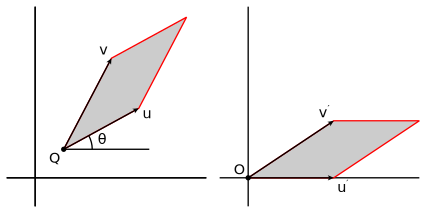
\includegraphics{4_a_parallelogram_rotated.eps}} 
%\resizebox{!}{1.75in}{\includegraphics{Parallelogram_original_b.eps}} \hspace{0.1in} \resizebox{!}{1.75in}{\includegraphics{Parallelogram_rotate_b.eps}}
    \caption{A parallelogram and a translated, rotated parallelogram.}
    \label{F:parallelograms}
  \end{center}
\end{figure}
If $\vu = [u_1 \ u_2]^{\tr}$ and $\vv = [v_1 \ v_2]^{\tr}$, then we will also represent $P(\vu,\vv)$ as $P\left( \left[ \begin{array}{cc}u_1&u_2 \\ v_1&v_2 \end{array} \right] \right)$. 

Since area is translation and rotation invariant, we can translate our parallelogram by $-\overrightarrow{OQ}$ to place its basepoint at the origin, then rotate by an angle $\theta$ (as shown at left in Figure \ref{F:parallelograms}. This transforms the vector $\vv$ to a vector $\vv'$ and the vector $\vu$ to a vector $\vu'$ as shown at right in Figure \ref{F:parallelograms}. With this in mind we can always assume that our parallelograms have one vertex at the origin, with $\vu$ along the $x$-axis, and $\vv$ in standard position. Now we can investigate how to calculate the area of a parallelogram. 

\begin{pactivity} \label{act:parallelogram_area} There are two situations to consider when we want to find the area of a parallelogram determined by vectors $\vu$ and $\vv$, both shown in Figure \ref{F:parallelogram_area}. The parallelogram will be determined by the lengths of these vectors.
\begin{figure}[ht]
  \begin{center}
 \resizebox{!}{1.0in}{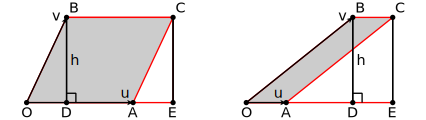
\includegraphics{4_a_parallelogram_area.eps}}  
%\resizebox{!}{0.85in}{\includegraphics{Parallelogram_area_1.eps}} \hspace{6pt} \resizebox{!}{0.85in}{\includegraphics{Parallelogram_area_2.eps}}
    \caption{Parallelograms formed by $\vu$ and $\vv$}
    \label{F:parallelogram_area}
  \end{center}
\end{figure}
\ba
\item In the situation depicted at left in Figure \ref{F:parallelogram_area}, use geometry to explain why $\Area(P(\vu,\vv)) = h |\vu|$. (Hint: What can we say about the triangles $ODB$ and $EAC$?)


\item In the situation depicted at right in Figure \ref{F:parallelogram_area}, use geometry to again explain why \\
$\Area(P(\vu,\vv)) = h |\vu|$. (Hint: What can we say about $\Area(AEC)$ and  $\Area(ODB)$?)

\ea

\end{pactivity}

The result of Project Activity \ref{act:parallelogram_area} is that the area of $P(\vu,\vv)$ is given by $h |\vu|$, where $h$ is the height of the parallelogram determined by dropping a perpendicular from the terminal point of $\vv$ to the line determined by the vector $\vu$. 

Now we turn to the question of how the determinant is related to area of a parallelogram. Our approach will use some properties of the area of $P(\vu, \vv)$. 

\begin{pactivity} \label{act:P_area_properties} Let $\vu$ and $\vv$ be vectors that determine a parallelogram in $\R^2$. 
\begin{figure}[ht]
  \begin{center}
 \resizebox{!}{1.0in}{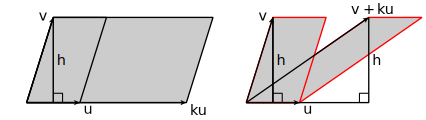
\includegraphics{4_a_parallelogram_shear.eps}} 
%\includegraphics[width=1.7in]{Parallelogram_stretch.eps} \hspace{6pt} \includegraphics[width=2.3in]{Parallelogram_shear.eps}
    \caption{Parallelograms formed by $k\vu$ and $\vv$ and by $\vu$ and $\vv+k\vu$.}
    \label{F:area_propertities}
  \end{center}
\end{figure}

\ba
\item Explain why 
\begin{equation} \label{eq:P_area_properties_1}
\Area(P(\vu,\vv)) = \Area(P(\vv,\vu))
\end{equation}


\item If $k$ is any scalar, then $k\vu$ either stretches or compresses $\vu$. Use this idea, and the result of Project Activity \ref{act:parallelogram_area}, to explain why
\begin{equation} \label{eq:P_area_properties_2}
\Area(P(k\vu,\vv)) = \Area(P(\vu,k\vv)) = |k| \Area(P(\vu,\vv))
\end{equation}
 for any real number $k$. A representative picture of this situation is shown at left in Figure \ref{F:parallelogram_area} for a value of $k > 1$. You will also need to consider what happens when $k < 0$. 
 
 
\item Finally, use the result of Project Activity \ref{act:parallelogram_area} to explain why
\begin{equation} \label{eq:P_area_properties_3}
\Area(P(\vu+k\vv,\vv)) = \Area(P(\vu,\vv+k\vu)) = \Area(P(\vu,\vv))
\end{equation}
for any real number $k$. A representative picture is shown at right in Figure \ref{F:area_propertities}.


\ea

\end{pactivity}


Properties (\ref{eq:P_area_properties_2}) and  (\ref{eq:P_area_properties_3}) will allow us to calculate the area of the parallelogram determined by vectors $\vu$ and $\vv$. 

\begin{pactivity} \label{act:det_area} Let $\vu = [u_1 \ u_2]^{\tr}$ and $\vv = [v_1 \ v_2]^{\tr}$. We will now demonstrate that 
\[\Area(P(\vu,\vv)) = \left|\det\left(\left| \begin{array}{cc} u_1&u_2\\v_1&v_2 \end{array} \right] \right)\right|.\]
Before we begin, note that if both $u_1$ and $v_1$ are $0$, then $\vu$ and $\vv$ are parallel. This makes $P(\vu, \vv)$ a line segment and so $\Area(P(\vu,\vv)) = 0$. But if $u_1 = v_1 = 0$, it is also the case that 
\[\det\left(\left| \begin{array}{cc} u_1&u_2\\v_1&v_2 \end{array} \right] \right) = u_1v_2-u_2v_1 = 0\]
as well. So we can assume that at least one of $u_1$, $v_1$ is not $0$. Since $P(\vu, \vv) = P(\vv, \vu)$, we can assume without loss of generality that $u_1 \neq 0$. 

\ba
\item Explain using properties (\ref{eq:P_area_properties_2}) and  (\ref{eq:P_area_properties_3}) as appropriate why
\[\Area(P(\vu,\vv)) =\Area\left(P\left(\vu, \left[0 \ v_2-\frac{v_1}{u_1}u_2\right] \right) \right).\]

\item Let $\vv_1 = \left[0 \ v_2-\frac{v_1}{u_1}u_2\right]^{\tr}$. Recall that our alternate representation of $P(\vu,\vv))$ allows us to write
\[\Area(P(\vu, \vv_1)) = \Area\left( P\left(  \left[ \begin{array}{cc} u_1&u_2 \\ 0&v_2-\frac{v_1}{u_1}u_2 \end{array} \right] \right) \right).\]
This should seem very suggestive. We are essentially applying the process of Gaussian elimination to our parallelogram matrix to reduce it to a diagonal matrix. From there, we can calculate the area. The matrix form should indicate the next step --  applying an operation to eliminate the entry in the first row and second column. To do this, we need to consider what happens if $v_2-\frac{v_1}{u_1}u_2 = 0$ and if $v_2-\frac{v_1}{u_1}u_2 \neq 0$. 
	\begin{enumerate}[i.]
	\item Assume that $v_2-\frac{v_1}{u_1}u_2 = 0$. Explain why $\Area(P(\vu,\vv)) = 0$. Then explain why $\Area(P(\vu,\vv)) = 0 = \det\left(\left[ \begin{array}{cc} u_1&u_2\\v_1&v_2 \end{array} \right]\right)$. 

	\item Now we consider the case when $v_2-\frac{v_1}{u_1}u_2 \neq 0$. Complete the process as in part (a), using properties (\ref{eq:P_area_properties_2}) and  (\ref{eq:P_area_properties_3}) (compare to Gaussian elimination) to continue to reduce the problem of calculating $\Area(P(\vu,\vv))$ to one of calculating $\Area(P(\ve_1, \ve_2))$. Use this process to conclude that 
\[\Area(P(\vu,\vv)) = \left| \det\left(\left[ \begin{array}{cc} u_1&u_2\\v_1&v_2 \end{array} \right]\right)\right|.\]


	\end{enumerate}

\ea

\end{pactivity}

We can apply the same arguments as above using rotations, translations, shearings, and scalings to show that the properties of area given above work in any dimension. Given vectors $\vu_1$, $\vu_2$, $\ldots$, $\vu_n$ in $\R^n$, we let 
\[P(\vu_1, \vu_2, \ldots, \vu_n) = \{\overrightarrow{OQ}+x_1 \vu_1 + x_2 \vu_2 + \cdots + x_n \vu_n : 0 \leq x_i \leq 1 \text{ for each } i\}.\]
If $n = 2$, then $P(\vu_1,\vu_2)$ is the parallelogram determined by $\vu_1$ and $\vu_2$ with basepoint $Q$. If $n = 3$, then $P(\vu_1, \vu_2, \vu_3)$ is the parallelepiped with basepoint $Q$ determined by $\vu_1$, $\vu_2$, and $\vu_3$. In higher dimensions the sets $P(\vu_1, \vu_2, \ldots,\vu_n)$ are called parallelotopes, and we use the notation $\Vol(P(\vu_1, \vu_2, \ldots,\vu_n))$ for their volume. The $n$-dimensional volumes of these paralleotopes satisfy the following properties:
\begin{align}
\Vol&(P(\vu_1, \vu_2, \ldots, \vu_{i-1}, \vu_i, \vu_{i+1}, \ldots, \vu_{j-1}, \vu_j, \vu_{j+1}, \ldots,\vu_n)) \notag \\
&= \Vol(P(\vu_1, \vu_2, \ldots, \vu_{i-1}, \vu_j, \vu_{i+1}, \ldots, \vu_{j-1}, \vu_i, \vu_{j+1}, \ldots,\vu_n))  \label{eq:vol_property_1} 
\end{align}
for any $i$ and $j$. 
%\begin{align} 
\begin{equation} 
\Vol(P(\vu_1,\vu_2, \ldots, \vu_{i-1}, k\vu_i, \vu_{i+1}, \ldots, \vu_n)) 
= |k| \Vol(P(\vu_1,\vu_2, \ldots, \vu_n)) \label{eq:vol_property_2} 
\end{equation}
%\end{align}
for any real number $k$ and any $i$. 
%\begin{align}
\begin{equation} 
\Vol(P(\vu_1,\vu_2, \ldots, \vu_{i-1}, \vu_{i}+k\vu_j, \vu_{i+1}, \ldots, \vu_n)) 
= \Vol(P(\vu_1,\vu_2, \ldots, \vu_n)) \label{eq:vol_property_3} 
\end{equation}
%\end{align}
for any real number $k$ and any distinct $i$ and $j$.

\begin{pactivity} \label{act:det_vol} We now show that $\Vol(P(\vu_1, \vu_2, \vu_3))$ is the absolute value of the determinant of $\left[ \begin{array}{c} \vu_1 \\ \vu_2 \\ \vu_3 \end{array} \right]$. For easier notation, let $\vu = [u_1 \ u_2 \ u_3]^{\tr}$, $\vv = [v_1 \ v_2 \ v_3]^{\tr}$, and $\vw = [w_1 \ w_2 \ w_3]^{\tr}$. As we argued in the 2-dimensional case, we can assume that all terms that we need to be nonzero are nonzero, and we can do so without verification. 
\ba
\item Explain how property (\ref{eq:vol_property_2}) shows that $\Vol(P(\vu, \vv, \vw))$ is equal to 
\[\Vol\left(P\left( \left[ \begin{array}{ccc} u_{1}&u_{2}&u_{3}
\\ 0&\frac{1}{u_1}(v_{2}u_1-v_{1}u_{2})&\frac{1}{u_1}(v_{3}u_1-v_{1}u_{3})\\ 0&\frac{1}{u_1}(w_{2}u_1-w_{1}u_{2})&\frac{1}{u_1}(w_{3}u_1-w_{1}u_{3}) \end {array} \right] \right)\right).\]
(Hint: Think about how these properties are related to row operations.)

\item Now let $\vv_1 = \left[ 0 \ \frac{1}{u_1}(v_{2}u_1-v_{1}u_{2}) \ \frac{1}{u_1}(v_{3}u_1-v_{1}u_{3})\right]^{\tr}$ and \\
$\vw_1 = \left[ 0 \ \frac{1}{u_1}(w_{2}u_1-w_{1}u_{2}) \ \frac{1}{u_1}(w_{3}u_1-w_{1}u_{3})\right]^{\tr}$. Explain how property (\ref{eq:vol_property_2}) shows that $\Vol(P(\vu, \vv, \vw))$ is equal to
\[\Vol\left(P\left( \left[ \begin{array}{ccc} u_{1}&u_{2}&u_{3}
\\ 0&\frac{1}{u_1}(v_{2}u_1-v_{1}u_{2})&\frac{1}{u_1}(v_{3}u_1-v_{1}u_{3})\\ 0&0&d \end {array} \right] \right)\right),\]
where 
\[d = \frac{1}{u_1v_2-u_2v_1}(u_1(v_2w_3-v_3w_2)-u_2(v_1w_3-v_{3}w_1)+u_3(v_1w_2-v_2w_1)).\]

\item Just as we saw in the 2-dimensional case, we can proceed to use the diagonal entries to eliminate the entries above the diagonal without changing the volume to see that 
\[\Vol(P(\vu, \vv, \vw)) = \Vol\left(P\left( \left[ \begin{array}{ccc} u_{1}&0&0
\\ 0&\frac{1}{u_1}(v_{2}u_1-v_{1}u_{2})&0\\ 0&0&d \end {array} \right] \right)\right).\]
Complete the process, applying appropriate properties to explain why 
\[\Vol(P(\vu, \vv, \vw)) = x \Vol(P(\ve_1, \ve_2, \ve_3))\]
for some constant $x$. Find the constant and, as a result, find a specific expression for $\Vol(P(\vu, \vv, \vw))$ involving a determinant. 


\ea

\end{pactivity}


Properties (\ref{eq:vol_property_1}), (\ref{eq:vol_property_2}), and (\ref{eq:vol_property_3}) involve the analogs of row operations on matrices, and we will prove algebraically that the determinant exhibits the same properties. In fact, the determinant can be uniquely defined by these properties. So in a sense, the determinant is an area or volume function. 



